\documentclass[11pt,reqno,final]{amsart}

\pdfcompresslevel=0
\pdfobjcompresslevel=0

\usepackage[dvipsnames]{xcolor}% adds colors
\usepackage{amsmath, amsthm}% {amsfonts, amssymb}

% New Characters
\usepackage[latin1]{inputenc}%
\usepackage[T1]{fontenc}

\usepackage{MnSymbol}
\usepackage[normalem]{ulem}% underlining

\usepackage[theoremfont, largesc]{newpxtext} % different text,math font
\usepackage{newpxmath}

\makeatletter
\DeclareMathRadical{\sqrtsign}{symbols}{112}{largesymbols}{112}
% \let\sqrt=\undefined
% \DeclareRobustCommand\sqrt{\@ifnextchar[\@sqrt{\mathpalette\@x@sqrt}]}
% \def\@x@sqrt#1#2{%
%  \setbox\z@\hbox{$\m@th#1\sqrtsign{\mkern1mu #2}$}
%  \mkern3mu\box\z@}
\makeatother




% Page Typesetting
\usepackage[final]{microtype}
\usepackage{relsize}
\usepackage[margin=1in]{geometry}
\usepackage{framed}
\usepackage{tikz}

\usepackage{csquotes}

\usepackage{setspace}
\onehalfspacing

\usepackage{hyperref}
\hypersetup{
  final,
  pdftitle={Math 135 - First Derivative Test},
  pdfauthor={Bonventre}, 
  linktoc=page,
  pagebackref,
  colorlinks=true,
  citecolor=PineGreen,
  linkcolor=PineGreen,
  linkbordercolor=PineGreen,
}


% Internal References

\usepackage[inline,shortlabels]{enumitem}

% \numberwithin{equation}{section} 
\numberwithin{figure}{section}

\usepackage[nameinlink,capitalise,noabbrev]{cleveref}

\crefname{equation}{}{} % get \cref to behave as \eqref

% \theoremstyle{plain} % bold name, italic text
\newtheorem{theorem}[equation]{Theorem}%
\newtheorem*{theorem*}{Theorem}%
\newtheorem{lemma}[equation]{Lemma}%
\newtheorem{proposition}[equation]{Proposition}%
\newtheorem{corollary}[equation]{Corollary}%
\newtheorem{conjecture}[equation]{Conjecture}%
\newtheorem*{conjecture*}{Conjecture}%
\newtheorem{claim}[equation]{Claim}%
\newtheorem{question}{Question}

\theoremstyle{definition} % bold name, plain text
\newtheorem{definition}[equation]{Definition}%
\newtheorem*{definition*}{Definition}%
\newtheorem{example}[equation]{Example}%
\newtheorem*{example*}{Example}%
\newtheorem{remark}[equation]{Remark}%
\newtheorem{notation}[equation]{Notation}%
\newtheorem{convention}[equation]{Convention}%
\newtheorem{assumption}[equation]{Assumption}%
\newtheorem{exercise}[question]{Exercise}

% ---------- macros
\newcommand{\set}[1]{\left\{#1\right\}}%
\newcommand{\sets}[2]{\left\{ #1 \;|\; #2\right\}}%
\newcommand{\longto}{\longrightarrow}%
\newcommand{\into}{\hookrightarrow}%
\newcommand{\onto}{\twoheadrightarrow}%

\usepackage{harpoon}
\newcommand{\vect}[1]{\text{\overrightharp{\ensuremath{#1}}}}

\newcommand{\del}{\partial}%

\newcommand{\ki}{\chi}
\newcommand{\ksi}{\xi}
\newcommand{\Ksi}{\Xi}

\newcommand{\dlim}{\displaystyle\lim}

% %%%%%%%%%%%%%%%%%%%%%%%%%%%%%%%%%%%%%%%%%%%%%%%%%%%%%%%%%%%%%%%%%%%%%%%%%%%%%%%%%%%%%%%%%%%%%%%%%%%%

\begin{document}


\begin{center}
        \textbf{\Large Math 135, Calculus 1, Fall 2020}\\[10pt]
        {\large 11-13: First Derivative Test (Section 4.3)}
\end{center}

\thispagestyle{empty}


\renewcommand{\thesection}{\Alph{section}}

% \vspace{-1pt}

The \textbf{derivative} $f'(x)$ of a function $y=f(x)$ gives:
\begin{itemize}
\item the slope of the tangent line
\item the instantaneous rate of change of $y$ with respect to $x$
\end{itemize}

The goal of today's class is understand how we can use the first derivative to get information about the original function.

Important result:
\begin{theorem}[Mean Value Theorem (MVT)]
        If a function $f$ is continuous on the closed interval $[a,b]$ and differentiable on $(a,b)$,
        then there exists an $x$-value $c \in (a,b)$ such that\\
        \begin{minipage}{0.5\textwidth}
                \[
                        f'(c) = \dfrac{f(b) - f(a)}{b-a}
                \]
                
                i.e.
                \begin{itemize}
                \item the \textit{instantaneous rate of change / slope of the tangent line} at $x = c$, and
                \item the \textit{average rate of change / slope of the secant line} over the interval $[a,b]$
                \end{itemize}
                are \textbf{equal}.        
        \end{minipage}
        \begin{minipage}{0.5\textwidth}
                \begin{center}
                        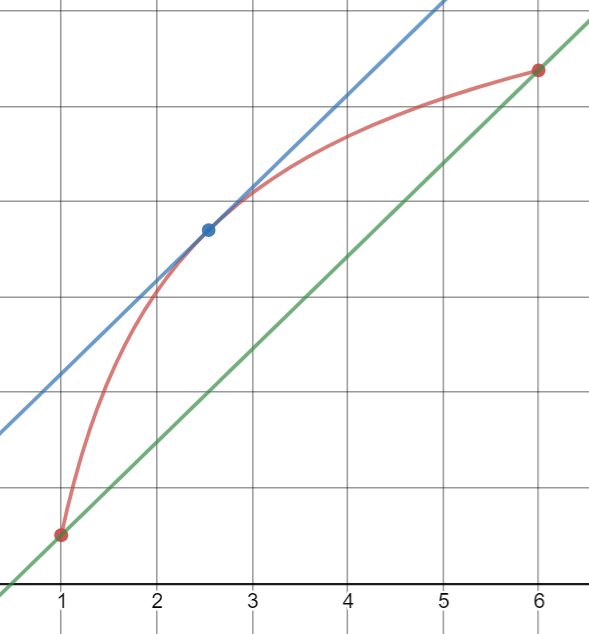
\includegraphics[width=2.3in]{11-13P_mvt.png}
                \end{center}
        \end{minipage}
\end{theorem}

Using the MVT, we can show the first derivative indicates whether the function is increasing, decreasing, or neither:
\begin{framed}
        \begin{gather*}
                \mbox{$f'(x) > 0$ for $x \in (a,b)$ $\Rightarrow$ $f$ is \textbf{increasing} on $(a,b)$}\\
                \mbox{$f'(x) < 0$ for $x \in (a,b)$ $\Rightarrow$ $f$ is \textbf{decreasing} on $(a,b)$}\\
                \mbox{$f'(c) = 0$ $\Rightarrow$ $c$ is a \textbf{critical point} of $f$}                  
        \end{gather*}
\end{framed}


We can use this to \textbf{classify} when a critical point is a \textbf{local max} or \textbf{local min}:

\subsection*{First Derivative Test} Suppose that $x = c$ is a critical point of $f$.

\begin{framed}
        \begin{gather*}
                \mbox{$f'(x)$ changes from $+$ to $-$ at $c$ \quad $\Rightarrow$ \quad $c$ is a \textbf{local max}}\\
                \mbox{$f'(x)$ changes from $-$ to $+$ at $c$ \quad $\Rightarrow$ \quad $c$ is a \textbf{local min}}\\
                \mbox{$f'(x)$ does not change sign at $c$ \quad $\Rightarrow$ \quad $c$ is \textbf{not a local extremum}}
        \end{gather*}
\end{framed}

\newpage

\begin{example}
        Let $f(x) = x^3 - 3x^2 - 45x + 5$.
        Together, let's find the critical points of $f$, and classify them using the First Derivative Test.
        On what interval(s) is $f$ increasing? decreasing?
        Use this information to sketch a graph of $f$.
        \vfill
\end{example}

\begin{exercise}
        For each of the following functions:
        \begin{itemize}
        \item Find the critical points of $f(x)$
        \item Find the intervals on which $f(x)$ is increasing or decreasing.
        \item Classify the critical points using the First Derivative Test
        \end{itemize}
        
        \begin{enumerate}[(a)]
        \item $f(x) = \dfrac{x^2 - 8x}{x+1}$
                \vfill
                \newpage
        \item $f(x) = (x^2-2x)e^x$
                \vfill
        \item $f(x) = 15x^3-x^5$
                \vfill
        \end{enumerate}
\end{exercise}


\end{document}
